\section{Belief Propagation} \label{BP}

The Warning Propagation algorithm is able to solve the decision problem and to compute valid assignments of SAT formulas. A different message passing method called the \emph{Belief Propagation} algorithm is able to determine the actual number of satisfying assignments and the fraction of those assignments where variables are restricted to fixed values. 

The messages sent in the BP algorithm are conditional probabilities $\mu \in [0, 1]$. The corresponding events are taken from the probability space built by all configurations of the  boolean variables $x_1, \ldots, x_n$. The used probability measure is a uniform distribution so for a SAT formula over $n$ variables each assignment has probability $2^{-n}$. \newline
This probability space can be restricted to only those configurations that satisfy a boolean formula $\mathcal{F}$. If there are $\mathcal{N}$ satisfying assignments the probability measure $P$ factorizes to $$P_{\mathcal{F}}(X) = P(X \; | \; X \text{ satisfies } \mathcal{F}) = \mathcal{N}^{-1} \prod_{a \in A} f_a(X)$$

where $A$ is the set of clauses in $\mathcal{F}$ and $f_a(X)$ the characteristic function of a clause $a$ that is $1$ if $X$ satisfies $a$ and $0$ if not.

The fraction of satisfying assignments where for example $x_1 = 1$ and $x_4 = 0$ can now be viewed as a marginal of $P_\mathcal{F}$ and computed using message passing techniques.

\subsection{Propagation Algorithm} \label{BPA}

\subsubsection{Messages}


The message $\mu_{a \rightarrow i}(x_i)$ sent from a factor $a$ to a variable $i$ is the probability that $a$ and all the factors behind $a$ are satisfied conditioned on $i$ taking the value $x_i$. 

%$\tau_{a \rightarrow i}$ is satisfied conditioned on $i$ taking the value $x_i$. 

The message $\mu_{i \rightarrow a}(x_i)$ sent in the opposite direction is the probability that $i$ takes the value $x_i$ in an assignment that satisfies $\tau_{i \rightarrow a}$.

\begin{example}
Let $\mathcal{F} = \underbrace{(x_1 \lor x_2 \lor \overline{x_3})}_a  \land \underbrace{(x_3 \lor x_4)}_b $.
\end{example}
\begin{figure}[h]
\centering

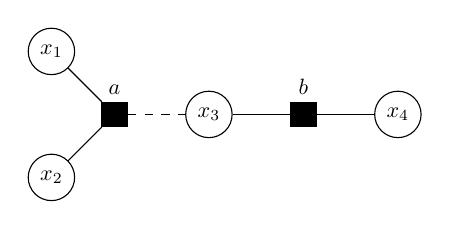
\begin{tikzpicture}[scale=0.8,transform shape]
   	\node[rectangle,draw=black, label = {$a$}, fill] (a) at (1,0) {$a$};
   	\node[rectangle,draw=black, label = {$b$}, fill] (b) at (4,0) {$a$};   
  \node[shape=circle,draw=black] (x1) at (0, 1) {$x_1$};
   
  \node[shape=circle,draw=black] (x2) at (0,-1) {$x_2$};
  \node[shape=circle,draw=black] (x3) at (2.5,0) {$x_3$};
  \node[shape=circle,draw=black] (x4) at (5.5,0) {$x_4$};
 


    
	\draw[-] (a) edge [right] node {} (x1);
	\draw[-] (a) edge [right] node {} (x2);
	\draw[-, dashed] (a) edge [right] node {} (x3);
	\draw[-] (b) edge [right] node {} (x3);
	\draw[-] (b) edge [right] node {} (x4);


\end{tikzpicture}
\end{figure}
The messages sent from $b$ to $x_3$ can be computed using only the definition: \newline
$\mu_{b \rightarrow 3}(1)$ is the probability that $(x_3 \lor x_4)$ is satisfied by an assignment where $x_3 = 1$ which is $1$. If $x_3 = 0$, only those assignments with $x_4 = 1$ satisfy $b$ so $\mu_{b \rightarrow 3}(0) = 0.5$. \newline
Out of all 14 configurations satisfying $(x_1 \lor x_2 \lor \overline{x_3})$ there are $8$ where $x_3 = 0$ and $6$ where $x_3 = 1$, so $\mu_{3 \rightarrow b}(0) = \frac{4}{7}, \, \mu_{3 \rightarrow b}(1) = \frac{3}{7}$. 

\subsubsection{Update Rules}


\begin{wrapfigure}{r}{0.3\textwidth}

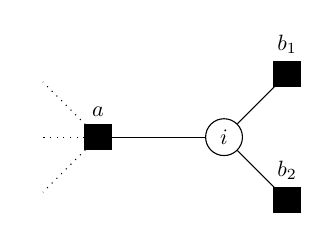
\begin{tikzpicture}[scale=0.8,transform shape]
   	\node[rectangle,draw=black, label = {$a$}, fill] (a) at (0,0) {$a$};
   	
\node[shape=circle,draw=black] (i) at (2,0) {$i$};   	
   	
   	\node[rectangle,draw=black, label = {$b_1$}, fill] (b1) at (3,1) {$a$};
   	\node[rectangle,draw=black, label = {$b_2$}, fill] (b2) at (3,-1) {$a$};

	\node[] (x1) at (-1,0) {};
	\node[] (x2) at (-1,1) {};
	\node[] (x3) at (-1,-1) {};

    \draw[dotted] (a) edge [right] node {} (x1);
    \draw[dotted] (a) edge [right] node {} (x2);
    \draw[dotted] (a) edge [right] node {} (x3);
	\draw[-] (a) edge [right] node {} (i);
	\draw[-] (i) edge [right] node {} (b1);
	\draw[-] (i) edge [right] node {} (b2);

\end{tikzpicture}
\end{wrapfigure}
$\mu_{b \rightarrow 3}(1)$ is the message   is passed to $a$ and tells the probability $i$ is $x_i$ considering only the factors on $i$'s side of the graph. \newline Through the tree structure of $\mathcal{F}$ these factors can be grouped into the subtrees $\tau_{b \rightarrow i}$ rooted in $i$'s neighbour factors $b_i \neq a$. These subgraphs are not connected and therefore independent to each other given the value of $i$.

$$\mu_{i\rightarrow a}(x_i) = P(x_i \; | \; \tau_{b_1 \rightarrow i} \land \ldots \land  \tau_{b_k \rightarrow i}) = \prod_b P(x_i \; | \; \tau_{b \rightarrow i}) = \prod_b \mu_{b\rightarrow i}$$


\subsection{Marginal Propabilities}

\subsection{Number of satisfying assignments}